\documentclass{article}[a4paper,12pt]

% Package Imports
\usepackage{amsmath}
\usepackage{graphicx}
\usepackage{subcaption}
\usepackage{lipsum}
\usepackage{hyperref}

% Config
\graphicspath{{../img/}}

% Preamble: Title Details
\title{Latex Tutorial}
\date{2023-10-25}
\author{Amanpreet Singh}

\begin{document}
  \pagenumbering{arabic}
  \maketitle %Insert Title
  \tableofcontents
  \newpage %Break Page

\section{Introduction}
This is the introduction section.
Tutorial being followed \href{http://www.latex-tutorial.com}{LaTeX-Tutorial}.

\subsection{Subsection}
This is a subsection.  

\subsubsection{Sub Subsection}
This is a sub-subsection.

\paragraph{Paragraph} 
This is a Paragraph.

\subparagraph{Sub Para}
This is a Sub Paragraph

\section{Features}

\subsection{Packages}

\paragraph{Equations}
Equations Package Example.
\begin{equation}
  f(x) = x^2
\end{equation}

\paragraph{Embedding}

...
This formula $f(x) = x^2$ is an embedding.
...


\paragraph*{Double Line}

\begin{equation*}
  1 + 2 = 3 
\end{equation*}
\begin{equation*}
  1 = 3 - 2
\end{equation*}

\begin{align*}
  1 + 2 &= 3\\
  1 &= 3 - 2
\end{align*}

Refering to Foot Note\footnote{\label{myfootnote}Tutorial footnote}.

\subsection{Formatting}

Various Formattings are Available.
\paragraph{Basic} Formatting Options using Tags.
\begin{enumerate}
  \item \textbf{Bold}
  \item \textit{Italics}
  \item \underline{Underline}
  \item \emph{Emphatic}
  \item `Single Quote'
  \item ``Double Quote''
  \item Special Chars, \verb|*`-$&|
\end{enumerate}

\paragraph{Alignment} Can be done using align block. 
\verb|*| Indicates not to put number for that Section.
\begin{align*}
  \text{Left Align}\\
  \text{Right aligned}
\end{align*}

\subsection{Math}

\paragraph{Fractions}

\begin{align*}
  f(x) &= x^2\\
  g(x) &= \frac{1}{x}\\
  F(x) &= \int^a_b \frac{1}{3}x^3
\end{align*}

\newpage

\subsection{Images}

\paragraph{Single}

Figure \ref{fig:sailboat} shows a boat. %Refers Label

\begin{figure}[h!]
  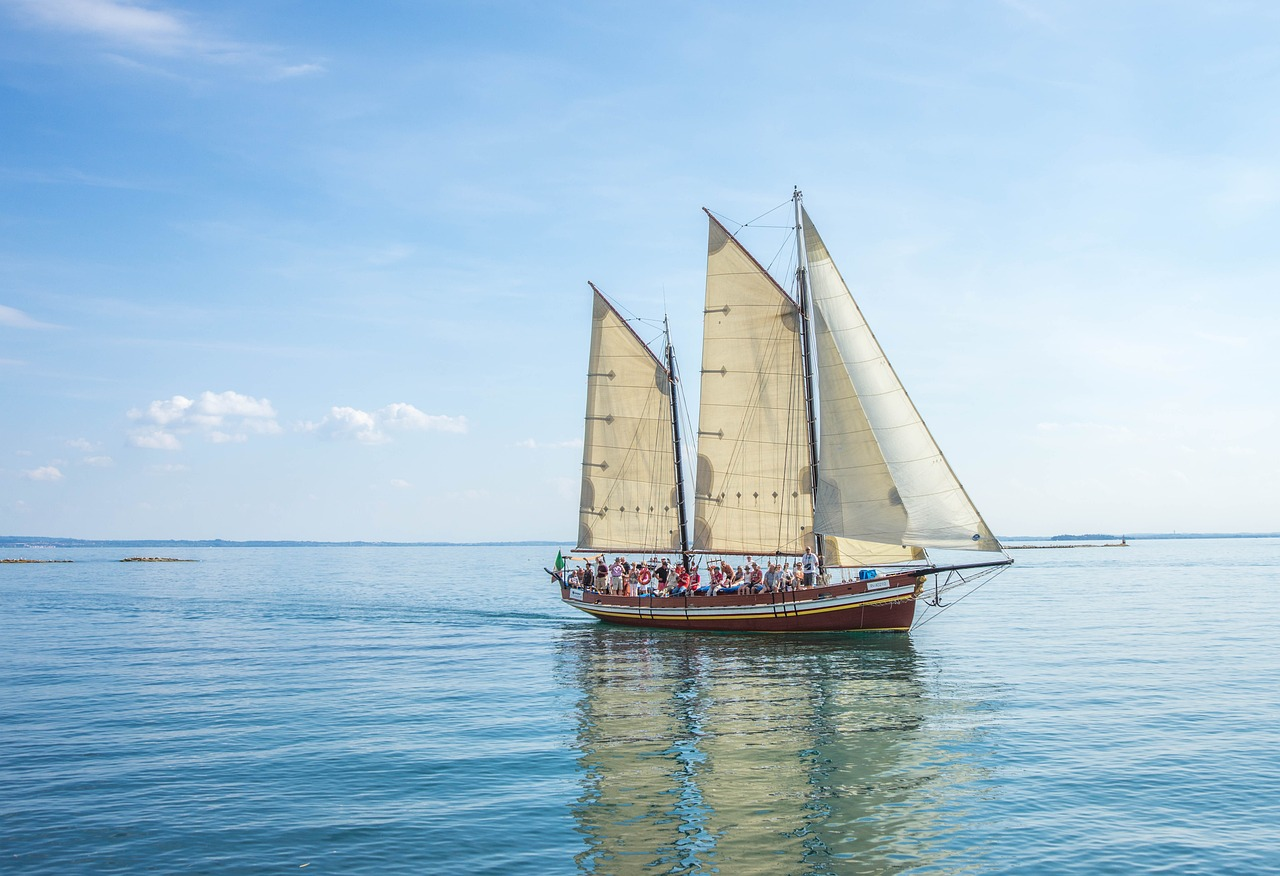
\includegraphics[width=\linewidth]{boat.jpg}
  \caption{Sail Boat.}
  \label{fig:sailboat} %Invisible Used for Reference
\end{figure}

\paragraph{Multiple}
Figure \ref{fig:coffee} shows how to place image side by side.

\subparagraph
There are two images aligned next to each other, their widths are both set to 0.4, yet they fill up the whole space.
You should always set this value to .1 less than you expect. If you want to align three images next to each other,
you should consecutively add three subfigures, each with a % ... 0.2\linewidth ...

\begin{figure}[h!]
  \centering
  \begin{subfigure}[b]{0.4\linewidth}
    
\includegraphics[width=\linewidth]{coffee.jpg}
    \caption{Coffee.}
  \end{subfigure}
  \begin{subfigure}[b]{0.4\linewidth}
    
\includegraphics[width=\linewidth]{coffee.jpg}
    \caption{More coffee.}
  \end{subfigure}
  \caption{Two Coffies}
  \label{fig:coffee}
\end{figure}

\paragraph{Cluster}
Figure \ref{fig:coffee3} shows how to place cluster of images.

\subparagraph
Notice images are Numbered Automatically.
I'm referring to footnote \ref{myfootnote}.

\begin{figure}[h!]
  \centering
  \begin{subfigure}[b]{0.2\linewidth}
    
\includegraphics[width=\linewidth]{coffee.jpg}
     \caption{Coffee.}
  \end{subfigure}
  \begin{subfigure}[b]{0.2\linewidth}
    
\includegraphics[width=\linewidth]{coffee.jpg}
    \caption{More coffee.}
  \end{subfigure}
  \begin{subfigure}[b]{0.2\linewidth}
    
\includegraphics[width=\linewidth]{coffee.jpg}
    \caption{Tasty coffee.}
  \end{subfigure}
  \begin{subfigure}[b]{0.5\linewidth}
    
\includegraphics[width=\linewidth]{coffee.jpg}
    \caption{Too much coffee.}
  \end{subfigure}
  \caption{Coffee Cluster}
  \label{fig:coffee3}
\end{figure}

\subsection{Tables}

\begin{align*}
  \href{https://tableconvert.com/latex-generator}{Table Generator}\\
  \href{https://latex-tutorial.com/tutorials/tables/}{Tutorial}
\end{align*}

\begin{table}[!ht]
  \centering
  \caption{Basic Table}
  \begin{tabular}{|l|l|}
  \hline
      \textbf{Heading 1} & \textbf{Heading 2} \\ \hline
      Hello & World \\ \hline
  \end{tabular}
  \label{tab:basic}
\end{table}

\begin{table}[h!]
  \begin{center}
    \caption{Alighned Table}
    \label{tab:alighned}
    \begin{tabular}{l|c|r} % <-- Alignments: 1st column left, 2nd middle and 3rd right, with vertical lines in between
      \textbf{Value 1} & \textbf{Value 2} & \textbf{Value 3}\\
      $\alpha$ & $\beta$ & $\gamma$ \\
      \hline
      1 & 1110.1 & a\\
      2 & 10.1 & b\\
      3 & 23.113231 & c\\
    \end{tabular}
  \end{center}
\end{table}

\subsection{Lists}
Lists are easy to create:
\paragraph{Bullets}

\begin{itemize}
  \label{lst:bullet}
  \item List entries start with the \verb|\item| command.
  \item Individual entries are indicated with a black dot, a so-called bullet.
  \item The text in the entries may be of any length.
  \item Below is an example of Nested List.
  \begin{itemize}
    \item Sub List 1
    \item \lipsum[1]
    \item Sub List 3
  \end{itemize}
\end{itemize}

\paragraph{Ordered}
This is an example of Ordered Lists.

\begin{enumerate}
  \label{lst:order}
  \item Latex is much more powerful than Markdown.
  \item It has lot more options as compared to markdown.
  \item Markdown syntax is simple but also limited.
  \begin{description}
    \item[Note:] This allows me to add such sections.
    \item[Tip!] Most of the complex Syntax is handled via IDE.
  \end{description}
\end{enumerate}

\begin{appendix}
  \listoffigures
  \listoftables
\end{appendix}

\end{document}